\documentclass[a4paper,29.6pt]{article}
%\documentclass[a4wide]{scrreprt}
\usepackage{graphicx}
%\usepackage{hyperref}
%\usepackage{palatino}
%\usepackage{hyperref}
%\usepackage{wrapfig}
%\usepackage{lipsum}
%\usepackage{mathtools}

%\parskip 7.2pt % sets spacing between paragraphs

%\renewcommand{\baselinestretch}{1.5} % Uncomment for 1.5 spacing between lines

%\parindent 0pt % sets leading space for paragraphs

\title {Project Report \\ Sensor Module Interfacing \\[10pt] Task: Ultrasonic Range Sensor Module Interfacing \\[25pt] Team members }
\author {Chayatan \and Mukilan A \and Shantanu Senguptha}

\begin{document}
\maketitle
\begin{center}
\begin{large}
Under the guidance of\\
\textbf{Prof. Kavi Arya\\and\\Parin Chedda}\\
\vspace{0.5in}
\end{large}
\end{center}
\begin{center}

\includegraphics[scale=0.32]{images/iitb}
\end{center}
\begin{center}
\begin{large}
Embedded and Real-Time Systems Laboratory \\
Department of Computer Science and Engineering \\
Indian Institute of Technology \\
Bombay \\
\end{large}
\end{center}
%\pagenumbering{roman} % Roman page number for toc
%\setcounter{page}{1} % Make it start with "ii"

\newpage
\tableofcontents
\newpage

\begin{abstract}
The project aims at interfacing ultrasonic range sensor with Fire Bird V educational robot. This additional module can be used for detection and ranging applications even in the harshest conditions. In this paper we will see about the basic MB 1310 ultrasonic range sensor module interfacing with Atmega 2560 in Fire Bird V robot. This will include the basic interfacing circuit, mounting, programming and calibration of the ultrasonic sensor.  
\end{abstract}

\section{Introduction}

\begin{large}
\hspace{.5in}Ultrasonic sensors are transceiver units which send and receive ultrasonic waves to detect and range objects in front of them. They are more reliable in harsh conditions than the sensors that use light waves. \\

MaxBotix AE1 (MB 1310) is an ultrasonic range sensor operated over low power 3.3V - 5V range which enables the sensor to detect objects from very small range up to long range. It is capable of detecting from 0 – 765cm and it can provide SONAR range information from 20 – 765 cm with 1cm resolution. The various interface output formats included are real time analog voltage envelope, analog voltage output and serial digital output.  
\\\\
A detailed description of the MB 1310 ultrasonic sensor module, interfacing circuit, mounting procedure, calibration technique and appropriate C code are explained below.\\

\end{large}
\begin{center}
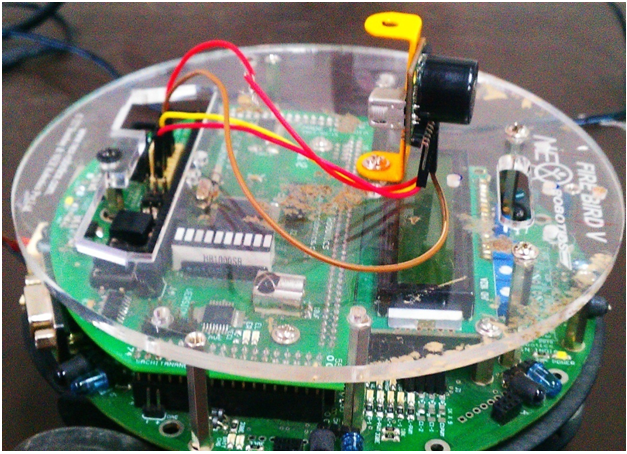
\includegraphics[scale=0.5]{1}
\end{center}


\newpage
\section{About MB-1310}
\subsection{Pin Configuration}
\begin{small}
%{!here}
%\begin{wrapfigure}{r}{0.5\textwidth}
  \begin{center}
    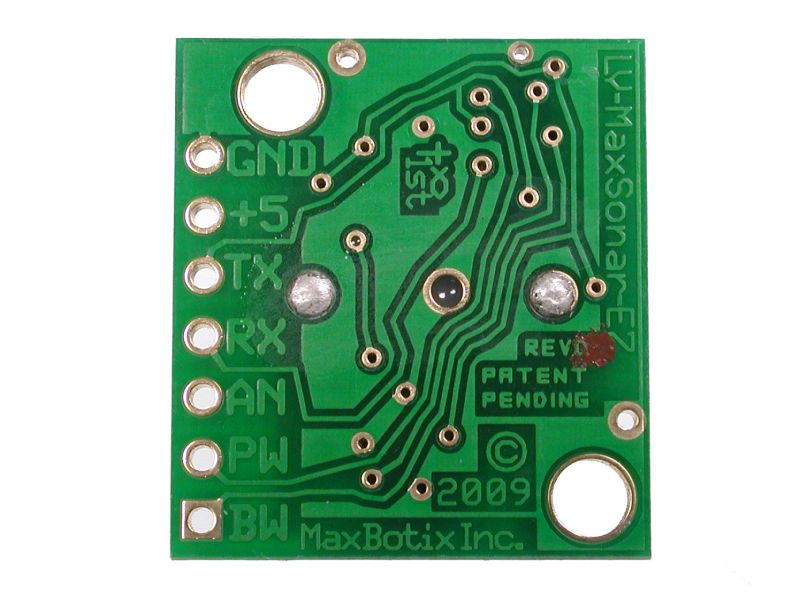
\includegraphics[width=0.48\textwidth]{3}
		\cite{app};
  \end{center}
  %\caption{A gull}
%\end{wrapfigure}
%\begin{center}
\noindent
\textbf{Pin 1:} This pin is internally pulled high.  It is left open or connected to the supply, so that it sends serial output through Pin5 in the RS-232 format.\\
\textbf{Pin 2:} PW pin gives the PWM representation of the range detected by the sensor. It is not used.\\
\textbf{Pin 3:} AN pin gives the analog output corresponding to the range detected by the sensor with a scaling factor of (Vcc/1024) per cm. This pin is used as the input to the ADC 15 slot in the Servo Pod.\\
\textbf{Pin 4:} RX pin – internally pulled high. This pin is used to either enable or disable the sensor. If it is kept open the sensor is always enabled. It is connected to the PB4 slot in the servo pod. This pin is kept high for 50ms enough to read the data.\\
\textbf{Pin 5:} TX pin – It transmits data in the RS-232 format when Pin  1 is high. It is not used.\\
The \textbf{$V_{cc}$} and \textbf{GND} pins are connected to the supply voltage 5V and ground respectively.\\



%\end{center}
The connections are then given to the servo pod slot provided in the Fire Bird V slot which will be discussed in the later section.\\\\
\end{small}

%\newpage
\section{Mounting and Interfacing the Sensor}
\subsection{Mounting Procedure}
\begin{small}
The sensor is bolted to a C joint which is in turn mounted on the Fire Bird V as shown in picture below. The pin-out connections are then given to the pins in the servo pod. This way of mounting gives the sensor its stability it needs to give correct readings while the bot is moving. It should be fixed in such a way that none of the robot's features affects the range of the sensor. It is advisable to tilt the sensor slightly upwards to prevent these hindrances. \\

\newpage
The picture shows how we have mounted the sensor on the robot.

\end{small}

\begin{center}
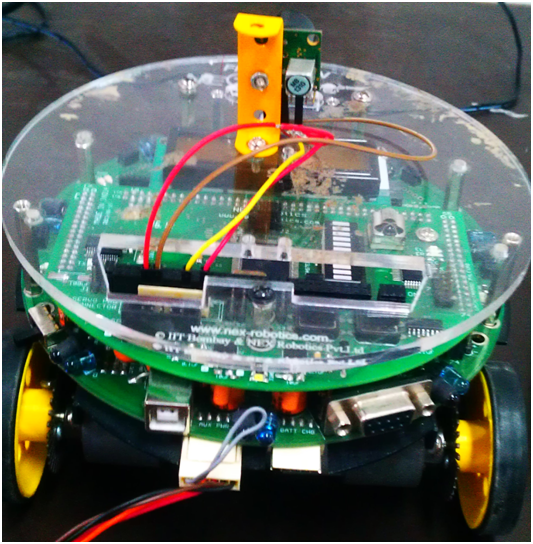
\includegraphics[scale=0.5]{2}
\end{center}
%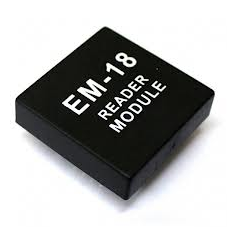
\includegraphics{em18}
%\cite{em18}\and
%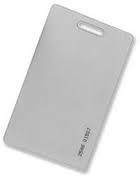
\includegraphics[scale=0.38]{tag}


%\hspace{1in}Fig1\hspace{2.2in}Fig2
%\end{small}

\subsection{Servo Pod Connections}
\begin{small}
The sensor is connected to ATMEGA 2560 through the servo pod slots provided in the Fire Bird V robot. The connections are given below:\\
\textbf{Pin 1:} ADC 14 connected to analog input (pin 3) of ultrasonic sensor.\\
\textbf{Pin 3:} PB4 is connected to the Rx pin of the senor. Controlling PB4 can enable or disable the sensor.\\
\textbf{Pin 6:} GND of the ultrasonic sensor.\\
\textbf{Pin 7:} Supply Voltage Vcc of the ultrasonic sensor.\\
The figure shows the servo pod connections.
\begin{center}
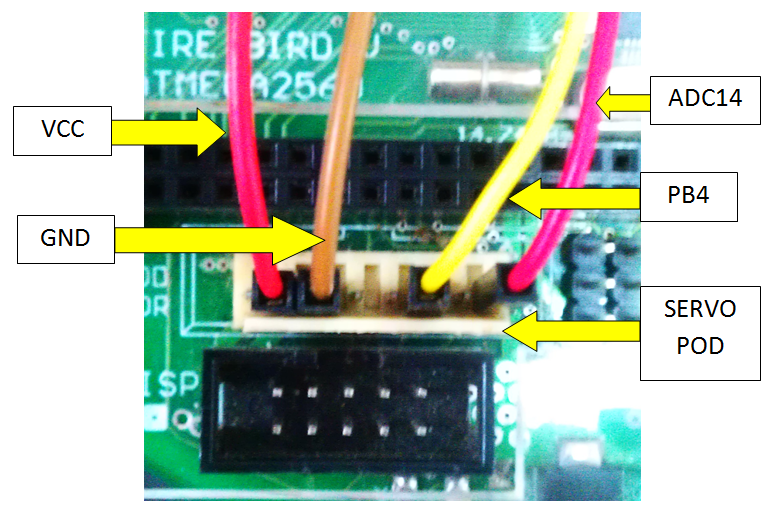
\includegraphics[scale=0.5]{4}
\end{center}

 

\end{small}

\section{Programming and Calibration}
\subsection{Algorithm}
\begin{small}
	The basic concept behind interfacing ultrasonic sensor is to receive the analog value from the sensor and store it in a register. The sensor sends 10 bit data. So the ADLAR register helps us to store it in the desired format in the ADCL and ADCH registers. This is discussed in the later section. Once the resultant value is got the value should be calibrated in such a way that it gives the exact values in centimeter. \\
	The various functions involved in the code and their functions are listed below.
	\begin{enumerate}
	\item \verb"'ADC_conversion()'" - receives the 10 bit analog value, converts it into a single 8 bit value and stores it in a variable 'a'.
	\item ultra() - will print the value in our desired format. The scaling factor included in this function will determine the unit in which we represent the data.
	\end{enumerate}
	\end{small}



\subsection{Calibration Procedure}
\begin{small}
The program is used to initialize the ADC 14 pin and receive the analog value from the sensor. Then the problem we face with the values is that it doesn't correspond to any particular value of measurement. It simply gives an analog value proportional to the distance measured. The calibration procedure to give the exact distance in centimeters is given below.\\
MB 1310 outputs analog voltage with a scaling factor of $(V_{cc}/1024)per\: cm$.
%\begin{align*}
	 $$Supply\: Voltage = 5V$$
		 $$Scaling\: factor= 5/1024 = 4.88mV/cm$$
		 ATMEGA 2560 ADC resolution for the 10 bit ADC it uses $$ Resolution = Vcc/(2^n) =5/1024$$ $$= 4.88mV/ADC Step$$
		 $$Distance\: in\: cm = ADC Steps * (4.88/4.88)$$ $$= ADC * 1$$ 
		 $$Scaling\: Factor = 1$$\\
		Thus the value got from the ADC pin must be multiplied with this scaling factor to get the value in centimeters. The scaling factor is 1 in this case. It need not be 1 always.
%\end{{align*}
\end{small}
\subsection{Determining ADC steps}
\begin{small}
The data registers of the ADC are ADCL and ADCH and the control bit ADLAR determines in which format the 10 bit value is stored in the data registers.\\
If ADLAR = 0;	the first eight bits are stored in ADCL and the remaining 2 bits are stored in ADC\\
If ADLAR=1;	ADC2-ADC9 are stored in ADCH and the lower order bits ADC0 and ADC1 are stored in the ADCL6 and ADCL7.  \\
We have used ADLAR = 1 and so we have followed the following steps to get the approximated ADC steps:\\
	Right shift the ADCL 6 locations and left shift ADCH by 2 locations and then OR both. 
	Now we have lost the Least Significant 2 bits. 
	And this resultant value should be considered as the ADC Step.\\
	\newpage
	The snippet shown below shows this ADC conversion process.
	\begin{center}
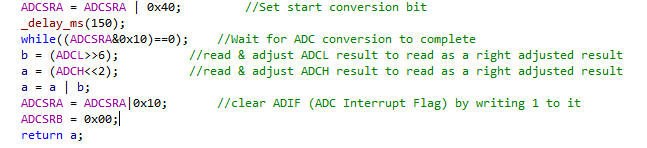
\includegraphics[scale=0.75]{adc}
\end{center}

\end{small}

\section{Header File}
\begin{small}
	The header file for the above created interfacing code can be created just by including a function which will return the value measured calibrated by the interfacing code.\\
	We have included a function called  \verb"'us_return()"'. This function will be called by the \verb"'ultra()"' in the interfacing code. The structure of the return function is given below.\\
	\verb"unsigned int us_return(void)"\\
\verb"{"\\
	\verb"return distance";\\
\verb"}"\\
	We can include the header file in any application folder and use the functions in it. The following figure shows one such simple program which has used the ultrasonic header file. \\ 
\begin{center}
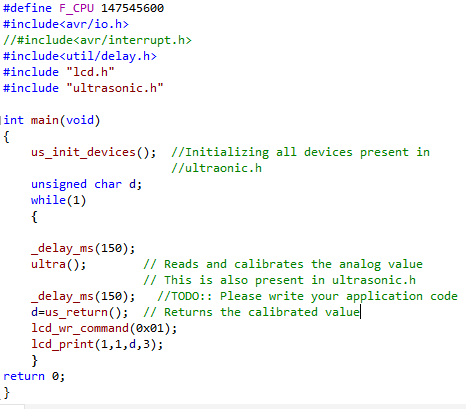
\includegraphics[scale=0.75]{app2}
\end{center}
	The function includes the 'ultrasonic.h' header file and in the body of the application program it has used 'ultra()' function. Thus the value the function has returned can be used in this application program.
\end{small}

\section{Output}
\begin{small}
The desired output will be in this format.
\begin{center}
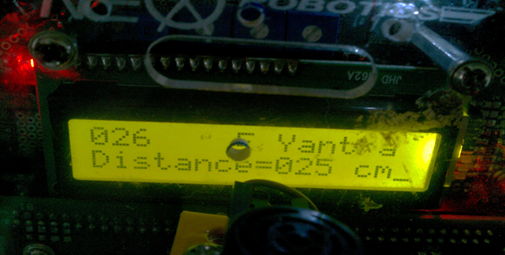
\includegraphics[scale=0.75]{5}
\end{center}
\end{small}

\section{Beam pattern}
The beam pattern will give the space in which the sensor will be able to detect any objects present in front of it. The values which we got from the experiment is listed below. The first column gives us  how far the object was placed from the base of the robot and the second column gives us the distance from the center of the sensor to the right upto which the object was detected. The beam pattern is symmetric along all direction.

%\begin{center}
\begin{table}[!h]

\TINY
\begin{tabular}{c c}
\toprule
\textbf{Distance from the sensor}&\textbf{Range from the center of the sensor}\\
\midrule
\textbf{20}&\textbf{7}\\
\textbf{80}&\textbf{21}\\
\textbf{140}&\textbf{30}\\
\textbf{200}&\textbf{35}\\
\textbf{260}&\textbf{34}\\
\textbf{320}&\textbf{35}\\
\textbf{380}&\textbf{33}\\
\textbf{440}&\textbf{35}\\
\textbf{500}&\textbf{34}\\
\textbf{560}&\textbf{36}\\
\textbf{620}&\textbf{30}\\
\textbf{680}&\textbf{25}\\
\textbf{740}&\textbf{13}\\
\bottomrule
\end{tabular}
\end{table}
%\end{center}


\newpage
\section{Applications}
\begin{small}
\begin{enumerate}
\item  They find use in applications such as humidifiers, sonar, medical ultra sonography, burglar alarms and non-destructive testing.
\item To measure tank or channel level, the sensor measures the distance to the surface of the fluid.
\item Ultrasonic sensors are used to detect movement of targets and to measure the distance to targets in many automated factories and process plants.
\item Nowadays ultrasonic sensors are widely used in automotive applications for park assist technology.
\end{enumerate}



\end{small}


%\newpage
\begin{thebibliography}{99}
\bibitem{app}
\url{https://solarbotics.com/product/35230/}

\end{thebibliography}
\end{document}